\chapter*{Introducción}
 
El artículo de Claude Shannon \textit{Mathematical Theory of Cryptography} (1945) y su ampliación posterior, \textit{Mathematical Theory of Communication} (1948) dieron a luz a dos disciplinas hoy plenamente establecidas, la teoría de información y la teoría de códigos.

El objetivo principal de estas disciplinas es el de establecer mecanismos de comunicación que sean \emph{eficientes} y \emph{fiables} en ambientes posiblemente hostiles.
La eficiencia requiere que la transmisión de la información no necesite de demasiados recursos, sean materiales o temporales.
Por otro lado, la fiabilidad requiere que el mensaje recibido en una comunicación sea lo más parecido posible, dentro de unos márgenes de tolerancia, al mensaje original.

La teoría de la información se encarga del estudio tanto de la representación de la información como de la capacidad que tienen los sistemas para transmitir y procesar la información. 
Por otra parte, la teoría de códigos se basa en los resultados de la teoría de la información para el diseño y desarrollo de modelos de transmisión de información mediante herramientas algebraicas.

\begin{figure}
  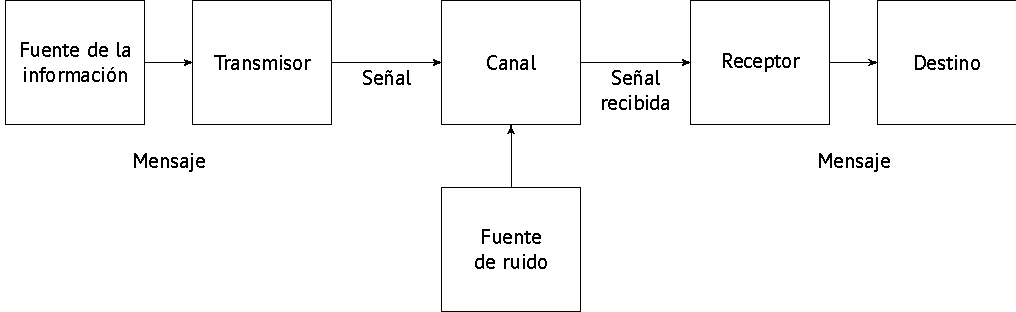
\includegraphics[width=\textwidth]{assets/shannon-communication-model.pdf}
  \caption*{Modelo de comunicación de Shannon}
\end{figure}

Esta disciplina no surge de la nada.
A lo largo de la historia el problema de codificar la información.
De hecho, el filósofo inglés Francis Bacon ya afirmó en el año 1623 que únicamente son necesarios dos símbolos para codificar toda la comunicación.

\blockquote[{\cite[30]{dyson_catedral_2015}}]{La transposición de dos letras en cinco emplazamientos bastará para dar 32 diferencias [y] por este arte se abre un camino por el que un hombre puede expresar y señalar las intenciones de su mente, a un lugar situado a cualquier distancia, mediante objetos ... capaces solo de una doble diferencia.}

Un código es una estructura algebraica.

Los avances recientes.

\section*{Enfoque}

El objetivo principal de este trabajo es el de exponer el algoritmo conocido como Peterson-Gorenstein-Zierler para códigos cíclicos sesgados.
Por tanto nos centramos en la exposición de las familias de códigos cíclicos.

\section*{Motivación}

El uso de anillos de polinomios de Ore nos permite obtener una mayor cantidad de códigos cíclicos.
El algoritmo PGZ para códigos BCH es interesante porque.
Por ello la adaptación para códigos cíclicos sesgados ofrece.

\section*{Objetivos}

Los objetivos de este trabajo son los siguientes. \begin{itemize}
  \item Estudio de las nociones básicas sobre Teoría de Códigos lineales.
  \item Estudio de las extensiones de Ore y de sus cocientes.
  \item Exponer el algoritmo de Peterson-Gorenstein-Zierler para códigos cíclicos sesgados.
  \item Implementación de sistemas de decodificación en Python usando Sage.
\end{itemize}

\section*{Esquema}

Primero fundamentos necesarios: capítulos 1 al 3.
Segundo entramos en detalle, explicamos el algoritmo PGZ para códigos BCH, introducimos los anillos de polinomios de Ore y los códigos cíclicos sesgados para finalmente introducir el algoritmo PGZ para códigos cíclicos sesgados.



